\documentclass{article}
\usepackage[T1]{fontenc}
\usepackage{lmodern}
\usepackage{graphicx}
\usepackage{amsmath,amssymb}
\usepackage[a4paper,margin=2cm]{geometry}
\usepackage[absolute,overlay]{textpos}
\setlength{\TPHorizModule}{1mm}
\setlength{\TPVertModule}{1mm}
\usepackage[indonesian]{babel}
\usepackage{hyperref}
\setlength{\emergencystretch}{2em}
% unit: Halaman 57

\begin{document}

% === Halaman 57 (llm) ===

If you need to know about RC4 encryption algorithm, please carefully read the instructions of this tool to set relevant parameters correctly.

\vspace{207.90mm}

Input Content

Terbanglah sampai ke angkasa setinggi bintang di langit

\begin{tabular}{|l|l|l|l|}
\hline
Password & selamat sore gaes & Charset & UTF-8 \\ \hline
In-Format & string & Out-Format & hex \\ \hline
\end{tabular}

RC4 Encrypt RC4 Decrypt Copy Clear

Output Result

5cc0adeadf45a1c2a0cb1b6527f95afa1a1cfb73d5dbd7173933f49139a227b088f5d06f0e35fd3efd2cb220bb4e971b1cbeae4fa2f694dc

% deskripsi: Screenshot antarmuka web alat enkripsi dan dekripsi RC4 yang menunjukkan input teks, password, pengaturan format, dan hasil output hex.
% bbox normalisasi: [0.0300, 0.2000, 0.9400, 0.9000]
\begin{textblock*}{191.10mm}(6.30mm,59.40mm)
\noindent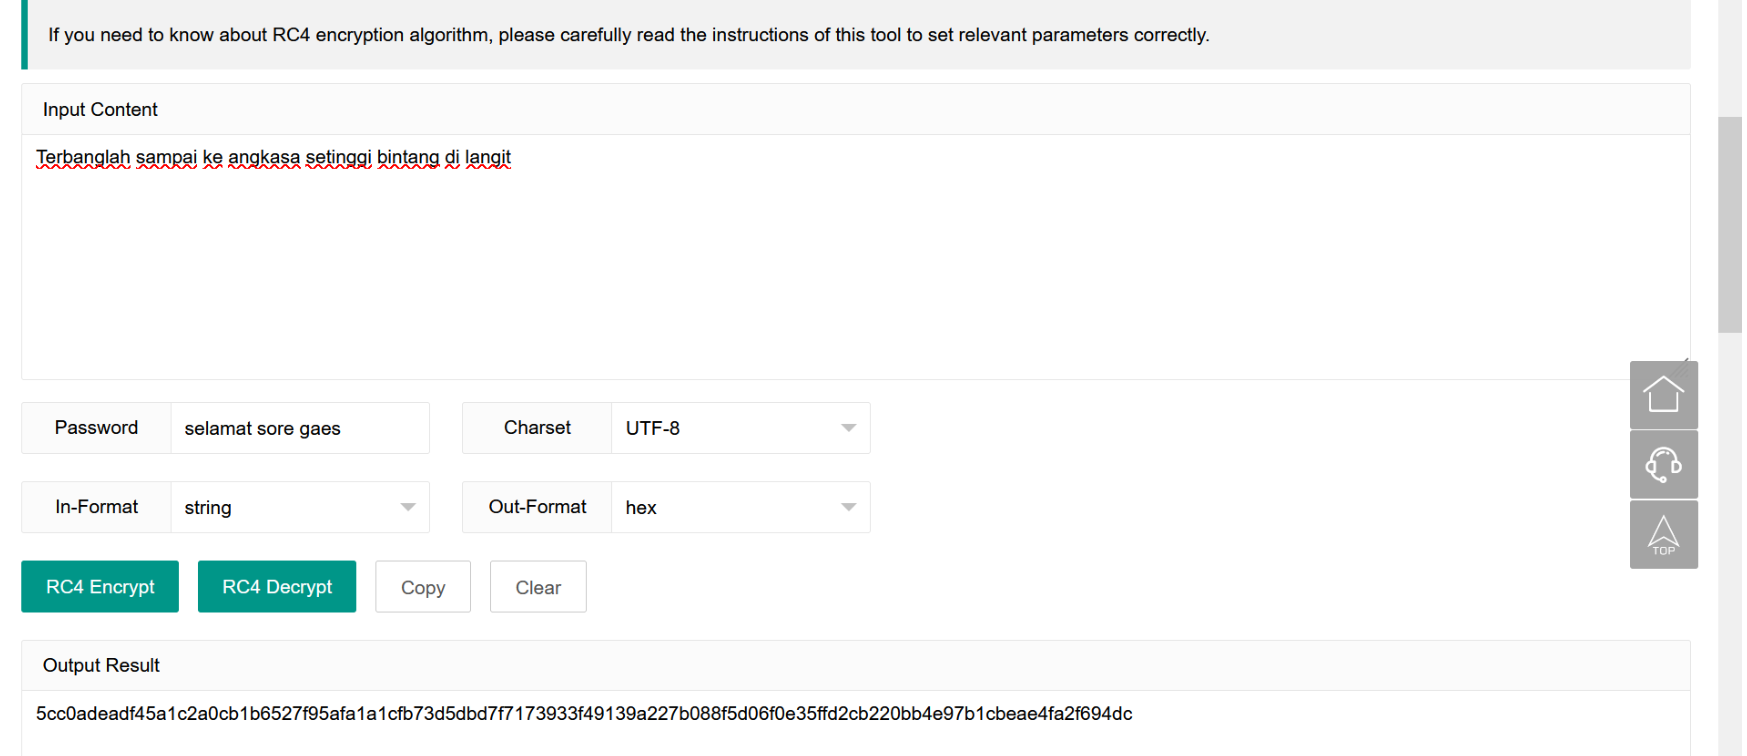
\includegraphics[width=191.10mm,height=207.90mm]{../../images/llm/page_057_img_01.png}%
\end{textblock*}

\end{document}
